\chapter{Anforderungen und Analyse}\label{kap:anforderunganalyse}

\section{Ziel der Arbeit}\label{sec:zielderarbeit}


Wie in der Einleitung \ref{kap:einleitung} beschrieben, soll 
ein CNN Basiertes System zur Wildtiererkennung entwickelt 
werden, das für dir Inferenz den Neural Compute Stick 2 verwendet.
Dabei sollte neben der reinen Erkennung auch eine Lokalisierung 
der erkannten Tiere im Bild stattfinden. Gängige Techniken dafür 
werden im nächsten Abschnitt erläutert.
\\
Dabei soll das Deep Learing Modell im Rahmen der gegebenen 
möglichkeiten und Limitierungen der Hardware möglichst 
genau und Robust sein, sodass es auch für die graustufen 
Bilder der Infrarot Kamera zuverlässig funktioniert.
Da eine erhöht Genauigkeit auch immer mit einer größeren
Latenz für der Inferenzzeit einhergeht war dies ein mit 
zu berücksichtigender Punkt.
\\
Neben training und evaluierung eines geeigneten Deep Learning Modells,
war die Implementierung der Anwendung, welche die Inferenz 
des Modells ausführt ein weiterer Bestandteil der Arbeit.
\\
Diese soll voll autonom auf dem Raspberry Pi laufen,
über eine mobile Netzwerk Verbindung verfügen und 
mittels eines geeigneten Kommunikations Protokolls die 
die erkannten und abgespeicherten Bilder an einen
Heim Pc senden.
Des weiteren sollte eine geeignete Kamera verwendet werden, die 
sowohl normale, als auch Infrarot Aufnahmen machen kann.


\section{Related Work}\label{sec:related_work}

Für die Objekterkennung werden häufig End-to-End Lösung verwendet,
Modelle die sowohl Klassifikation als auch Lokalisierung 
durchführen.
Diese verwenden meist eines der im Abschnitt 
\ref{subsubsec:architecture} erläuterten Basis CNNs als  
\textit{Feature Extractor} und darauf aufbauend ein Framework
für die Lokalisierung. 

Diese lassen sich, wie in \cite{wengObjectDetectionPart2018} beschrieben,
in einstufige und zweistufige Verfahren gliedern. 

\subsubsection{Region Based CNNs}
Bei den zweistufigen
handelt es sich um Regionbased CNNs, die Regionen für
mögliche Box Locations mithilfe RPN (Region Proposia Network)
oder selective search verfahren finden soll, um diese dann
zu klassifizieren bzw box regression. Die aktuellste Version 
davon ist das in Abbildung \ref{fig:faster_rcnn} schematisch 
dargestellte \textit{Faster R-CNN} \cite{renFasterRCNNRealTime2016a}


\begin{figure}[H]
    \centering
    \label{fig:faster_rcnn}
    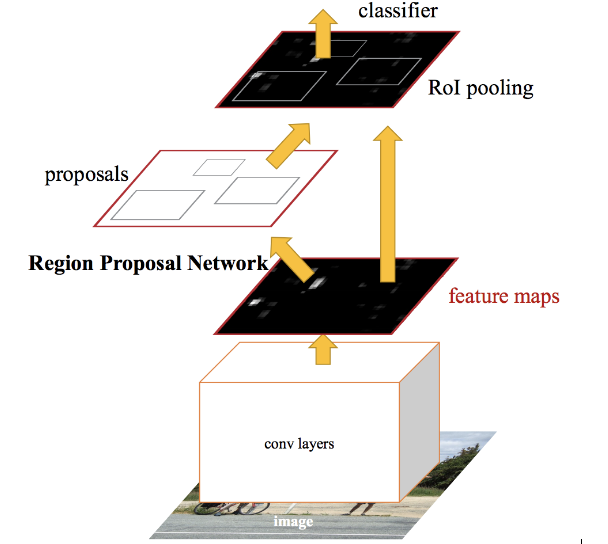
\includegraphics[width=0.5\textwidth]{faster_rcnn.png}
    \caption{Faster R-CNN, \cite{renFasterRCNNRealTime2016a}}
\end{figure}


\subsubsection{Single Shot Detectoren}
Einstufige Verfahren wie Single Shot Detectoren (SSD) 
führen die lokalisierung zusammen mit dem Feature Extractor 
aus, indem verschiedene scalierungen/ausmaße der Convolutional 
Layer in den Classifier/Regressor gegeben werden.
Dadurch sind diese wie in Abbildung \ref{fig:speed_acc}
zu erkennen ist, zwar schneller, jedoch auch ungenauer.


\begin{minipage}[t]{0.5\textwidth}
    \centering
    \label{fig:faster_rcnn}
    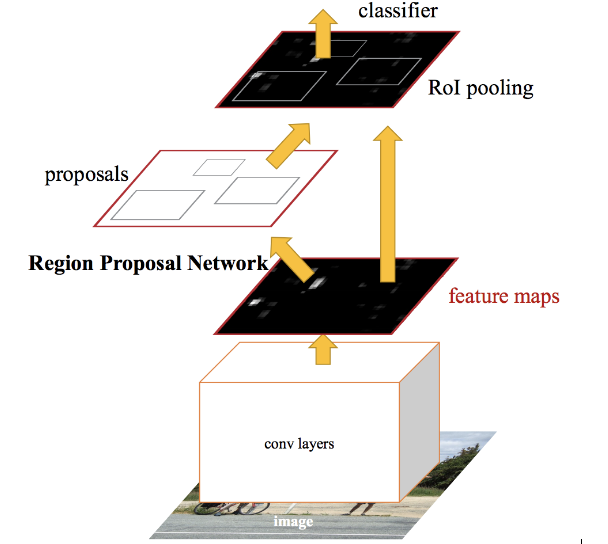
\includegraphics[width=0.67\textwidth]{faster_rcnn.png}
    \captionof{figure}{Faster R-CNN, \cite{renFasterRCNNRealTime2016a}}
\end{minipage}
\begin{minipage}[t]{0.5\textwidth}
    \centering
    \label{fig:speed_acc}
    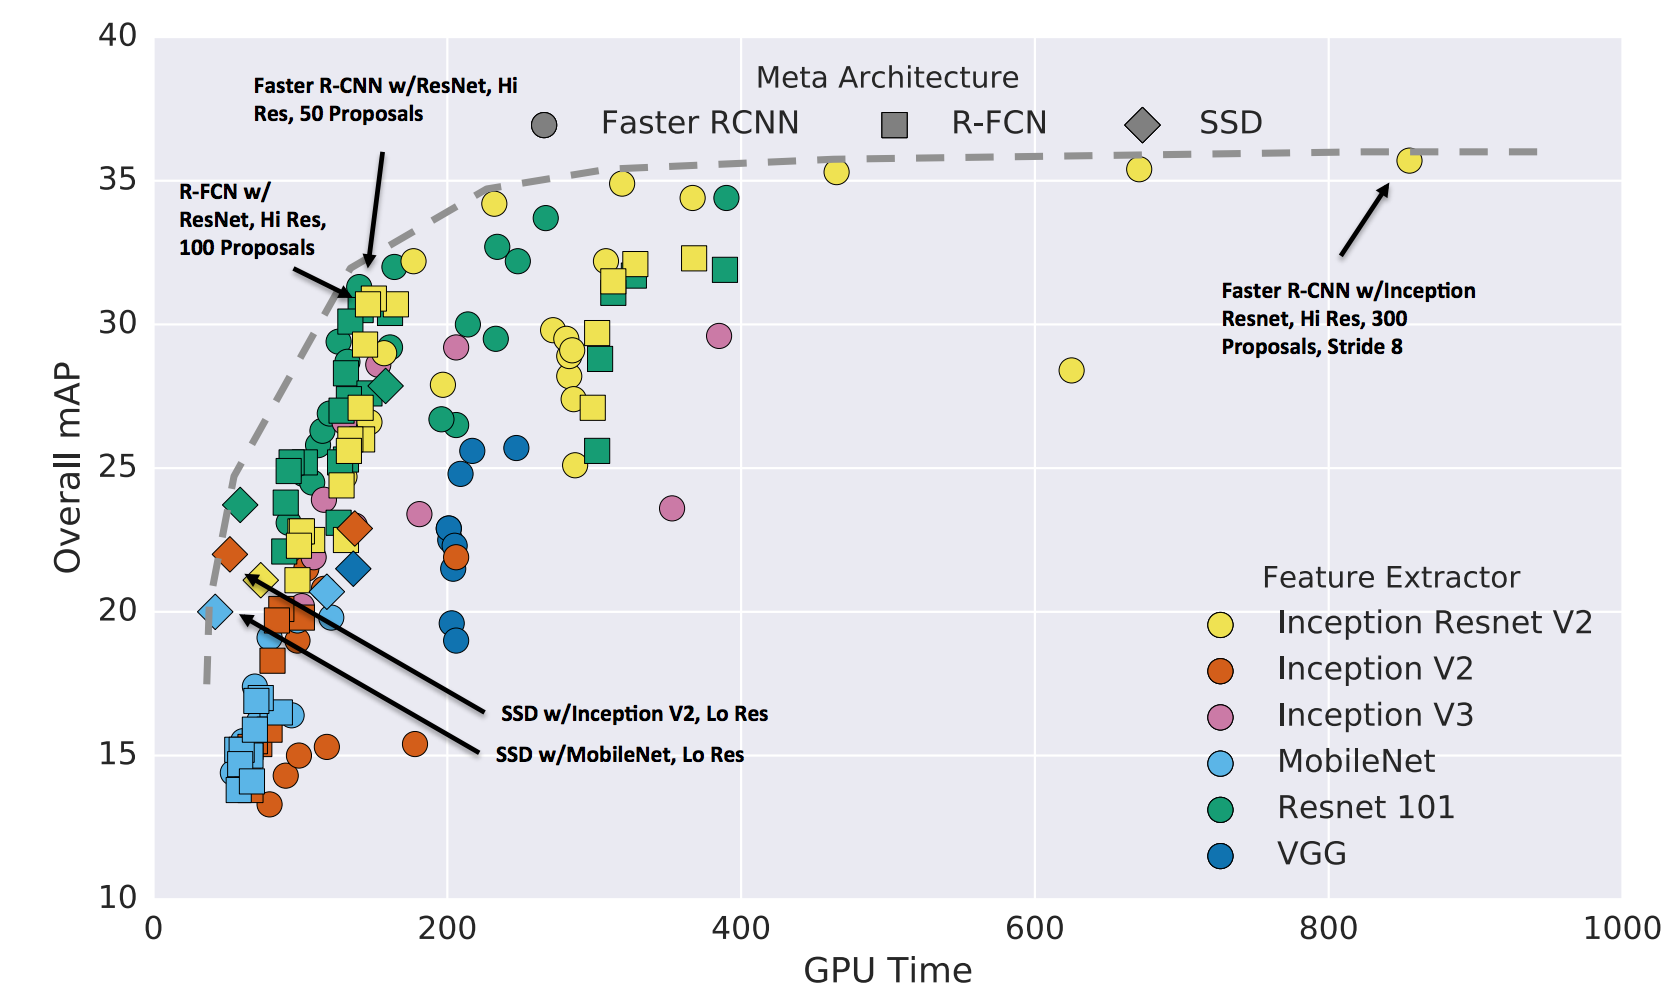
\includegraphics[width=\textwidth]{speed_acc_comp.png}
    \captionof{figure}{Geschw vs Genauigkeit, \cite{huangSpeedAccuracyTradeOffs2017}}
\end{minipage}